\subsection{Alternative synthesis of S$_N$2 conjugates}

Given the side-reactions and low yields associated with the literate synthesis of the S$_N$2 conjugates proposed by Ganguly et. al\cite{Ganguly2011}, we investigated a second synthesis, building up the linker on the ciprofloxacin side before coupling with the head group (see \ref{sch:HOcy5NH4CipMeRR_synth}).

\begin{scheme}[H]
	\begin{center}
		\schemeref[CipMe]{cmpd:CipMe}
		\schemeref[tBu4Br]{cmpd:tBu4Br}
		\schemeref[tBu4CipMe]{cmpd:tBu4CipMe}
		\schemeref[4CipMe]{cmpd:4CipMe}
		\schemeref[HOcy5NH4CipMe]{cmpd:HOcy5NH4CipMe}
		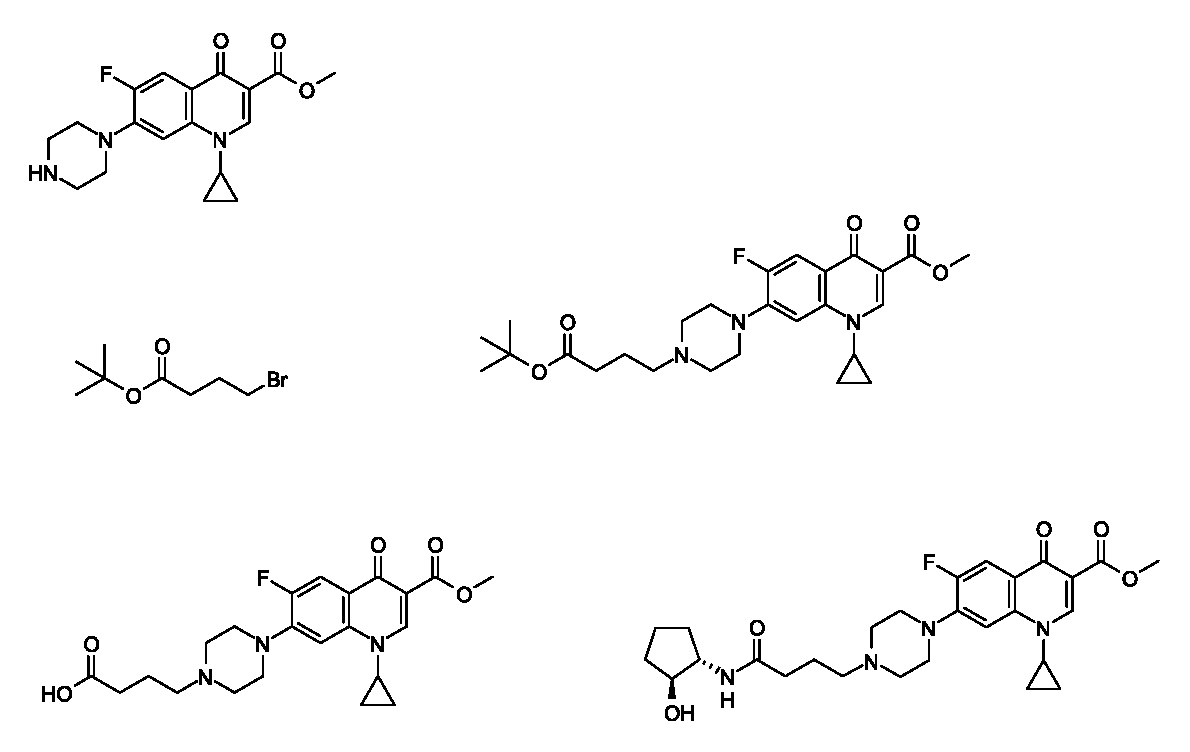
\includegraphics[scale=1]{HOcy5NH4CipMeRR_synth}
		\caption{Synthesis of \compound{cmpd:HOcy5NH4CipMeRR}. 
		a) . 
		\label{sch:HOcy5NH4CipMeRR_synth}}
	\end{center}
\end{scheme}